%! TEX encoding = utf8
\chapter{Odpowiedzi skokowe}

\section{Opowiedzi skokowe}
Rozważamy 5 różnych wartości skoku: \num{0,1}, \num{0,15}, \num{0,2}, \num{0,25}, \num{0,3}.

\begin{figure}[H]
\centering
% This file was created by matlab2tikz.
%
%The latest updates can be retrieved from
%  http://www.mathworks.com/matlabcentral/fileexchange/22022-matlab2tikz-matlab2tikz
%where you can also make suggestions and rate matlab2tikz.
%
\definecolor{mycolor1}{rgb}{0.00000,0.44700,0.74100}%
\definecolor{mycolor2}{rgb}{0.85000,0.32500,0.09800}%
\definecolor{mycolor3}{rgb}{0.92900,0.69400,0.12500}%
\definecolor{mycolor4}{rgb}{0.49400,0.18400,0.55600}%
\definecolor{mycolor5}{rgb}{0.46600,0.67400,0.18800}%
%
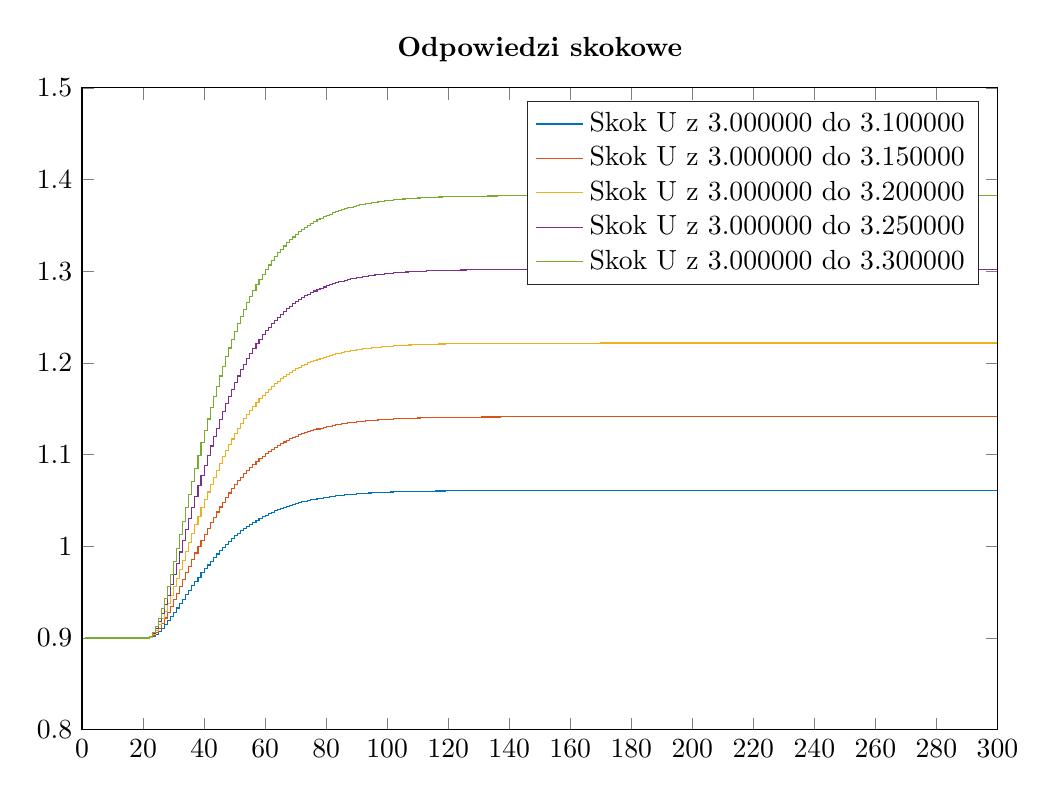
\begin{tikzpicture}

\begin{axis}[%
width=4.577in,
height=3.209in,
at={(0.768in,0.433in)},
scale only axis,
xmin=0,
xmax=300,
ymin=0.8,
ymax=1.5,
axis background/.style={fill=white},
title style={font=\bfseries},
title={Odpowiedzi skokowe},
legend style={legend cell align=left, align=left, draw=white!15!black}
]
\addplot[const plot, color=mycolor1] table[row sep=crcr] {%
1	0.9\\
2	0.9\\
3	0.9\\
4	0.9\\
5	0.9\\
6	0.9\\
7	0.9\\
8	0.9\\
9	0.9\\
10	0.9\\
11	0.9\\
12	0.9\\
13	0.9\\
14	0.9\\
15	0.9\\
16	0.9\\
17	0.9\\
18	0.9\\
19	0.9\\
20	0.9\\
21	0.9\\
22	0.90052911\\
23	0.902002516201\\
24	0.904264895040259\\
25	0.907179871020595\\
26	0.910627962037437\\
27	0.914504734035138\\
28	0.918719144461368\\
29	0.923192055952194\\
30	0.927854903459593\\
31	0.932648499644957\\
32	0.937521964821955\\
33	0.942431769054246\\
34	0.947340875210701\\
35	0.952217972864635\\
36	0.957036793904703\\
37	0.96177550161309\\
38	0.966416145770208\\
39	0.970944177072121\\
40	0.975348014804627\\
41	0.979618662312712\\
42	0.983749365341996\\
43	0.987735308815067\\
44	0.991573348045132\\
45	0.995261770786663\\
46	0.998800086881593\\
47	1.00218884258381\\
48	1.00542945693751\\
49	1.00852407784915\\
50	1.01147545573171\\
51	1.01428683281474\\
52	1.01696184640842\\
53	1.01950444458486\\
54	1.0219188128977\\
55	1.02420931090367\\
56	1.02638041737792\\
57	1.02843668323069\\
58	1.03038269123652\\
59	1.03222302178155\\
60	1.03396222391796\\
61	1.03560479109122\\
62	1.03715514097323\\
63	1.03861759889624\\
64	1.03999638443721\\
65	1.0412956007517\\
66	1.04251922630079\\
67	1.04367110865423\\
68	1.04475496008867\\
69	1.04577435473192\\
70	1.0467327270325\\
71	1.04763337135964\\
72	1.04847944256153\\
73	1.04927395733033\\
74	1.05001979624045\\
75	1.05071970634301\\
76	1.05137630421413\\
77	1.05199207936719\\
78	1.05256939795115\\
79	1.053110506667\\
80	1.05361753684359\\
81	1.05409250862209\\
82	1.05453733520564\\
83	1.05495382713671\\
84	1.05534369657075\\
85	1.05570856151918\\
86	1.05604995003936\\
87	1.05636930435292\\
88	1.05666798487717\\
89	1.05694727415721\\
90	1.05720838068888\\
91	1.057452442625\\
92	1.05768053135919\\
93	1.05789365498325\\
94	1.05809276161549\\
95	1.05827874259872\\
96	1.05845243556741\\
97	1.0586146273848\\
98	1.05876605695114\\
99	1.058907417885\\
100	1.05903936108011\\
101	1.05916249714066\\
102	1.05927739869816\\
103	1.05938460261335\\
104	1.05948461206693\\
105	1.05957789854269\\
106	1.05966490370728\\
107	1.05974604119021\\
108	1.05982169826842\\
109	1.05989223745912\\
110	1.05995799802512\\
111	1.06001929739631\\
112	1.06007643251132\\
113	1.06012968108298\\
114	1.0601793027914\\
115	1.06022554040799\\
116	1.06026862085422\\
117	1.06030875619803\\
118	1.06034614459156\\
119	1.0603809711529\\
120	1.06041340879513\\
121	1.06044361900535\\
122	1.06047175257646\\
123	1.06049795029434\\
124	1.06052234358293\\
125	1.0605450551095\\
126	1.06056619935251\\
127	1.06058588313412\\
128	1.06060420611942\\
129	1.06062126128432\\
130	1.06063713535402\\
131	1.06065190921369\\
132	1.06066565829307\\
133	1.06067845292662\\
134	1.06069035869055\\
135	1.06070143671833\\
136	1.06071174399582\\
137	1.06072133363737\\
138	1.06073025514402\\
139	1.06073855464497\\
140	1.0607462751233\\
141	1.06075345662693\\
142	1.06076013646584\\
143	1.06076634939626\\
144	1.06077212779279\\
145	1.06077750180919\\
146	1.06078249952847\\
147	1.06078714710314\\
148	1.06079146888607\\
149	1.06079548755266\\
150	1.06079922421492\\
151	1.06080269852789\\
152	1.06080592878893\\
153	1.06080893203039\\
154	1.06081172410605\\
155	1.06081431977174\\
156	1.06081673276054\\
157	1.06081897585291\\
158	1.06082106094204\\
159	1.06082299909488\\
160	1.06082480060889\\
161	1.0608264750651\\
162	1.0608280313774\\
163	1.06082947783864\\
164	1.06083082216344\\
165	1.06083207152822\\
166	1.06083323260836\\
167	1.06083431161293\\
168	1.06083531431697\\
169	1.0608362460916\\
170	1.06083711193207\\
171	1.06083791648382\\
172	1.06083866406682\\
173	1.06083935869823\\
174	1.06084000411341\\
175	1.06084060378563\\
176	1.06084116094426\\
177	1.06084167859183\\
178	1.06084215951987\\
179	1.0608426063236\\
180	1.06084302141568\\
181	1.06084340703898\\
182	1.06084376527842\\
183	1.06084409807209\\
184	1.06084440722148\\
185	1.06084469440107\\
186	1.06084496116724\\
187	1.06084520896657\\
188	1.06084543914352\\
189	1.06084565294761\\
190	1.06084585154011\\
191	1.0608460360002\\
192	1.06084620733082\\
193	1.06084636646393\\
194	1.06084651426561\\
195	1.06084665154063\\
196	1.0608467790368\\
197	1.06084689744897\\
198	1.06084700742279\\
199	1.06084710955815\\
200	1.06084720441243\\
201	1.06084729250348\\
202	1.06084737431244\\
203	1.06084745028631\\
204	1.06084752084039\\
205	1.06084758636049\\
206	1.06084764720502\\
207	1.06084770370696\\
208	1.06084775617563\\
209	1.06084780489836\\
210	1.06084785014209\\
211	1.06084789215474\\
212	1.06084793116666\\
213	1.06084796739176\\
214	1.06084800102878\\
215	1.06084803226229\\
216	1.06084806126375\\
217	1.0608480881924\\
218	1.06084811319614\\
219	1.06084813641234\\
220	1.0608481579686\\
221	1.06084817798342\\
222	1.06084819656686\\
223	1.06084821382113\\
224	1.06084822984116\\
225	1.06084824471511\\
226	1.06084825852486\\
227	1.06084827134644\\
228	1.06084828325047\\
229	1.06084829430253\\
230	1.0608483045635\\
231	1.06084831408995\\
232	1.06084832293439\\
233	1.06084833114558\\
234	1.06084833876881\\
235	1.06084834584614\\
236	1.0608483524166\\
237	1.06084835851645\\
238	1.06084836417938\\
239	1.06084836943663\\
240	1.06084837431725\\
241	1.06084837884818\\
242	1.06084838305445\\
243	1.0608483869593\\
244	1.06084839058432\\
245	1.06084839394953\\
246	1.06084839707354\\
247	1.06084839997362\\
248	1.0608484026658\\
249	1.06084840516498\\
250	1.06084840748499\\
251	1.06084840963864\\
252	1.06084841163787\\
253	1.06084841349374\\
254	1.06084841521652\\
255	1.06084841681574\\
256	1.06084841830026\\
257	1.0608484196783\\
258	1.06084842095749\\
259	1.06084842214492\\
260	1.06084842324716\\
261	1.06084842427033\\
262	1.06084842522008\\
263	1.06084842610169\\
264	1.06084842692004\\
265	1.06084842767967\\
266	1.06084842838479\\
267	1.0608484290393\\
268	1.06084842964684\\
269	1.06084843021077\\
270	1.06084843073423\\
271	1.06084843122011\\
272	1.06084843167112\\
273	1.06084843208975\\
274	1.06084843247832\\
275	1.060848432839\\
276	1.06084843317379\\
277	1.06084843348454\\
278	1.06084843377298\\
279	1.0608484340407\\
280	1.06084843428921\\
281	1.06084843451986\\
282	1.06084843473396\\
283	1.06084843493268\\
284	1.06084843511712\\
285	1.06084843528833\\
286	1.06084843544723\\
287	1.06084843559472\\
288	1.06084843573162\\
289	1.06084843585869\\
290	1.06084843597662\\
291	1.06084843608609\\
292	1.06084843618769\\
293	1.060848436282\\
294	1.06084843636952\\
295	1.06084843645077\\
296	1.06084843652617\\
297	1.06084843659616\\
298	1.06084843666111\\
299	1.0608484367214\\
300	1.06084843677736\\
};
\addlegendentry{Skok U z 3.000000 do 3.100000}

\addplot[const plot, color=mycolor2] table[row sep=crcr] {%
1	0.9\\
2	0.9\\
3	0.9\\
4	0.9\\
5	0.9\\
6	0.9\\
7	0.9\\
8	0.9\\
9	0.9\\
10	0.9\\
11	0.9\\
12	0.9\\
13	0.9\\
14	0.9\\
15	0.9\\
16	0.9\\
17	0.9\\
18	0.9\\
19	0.9\\
20	0.9\\
21	0.9\\
22	0.900793665\\
23	0.9030037743015\\
24	0.906397342560389\\
25	0.910769806530893\\
26	0.915941943056156\\
27	0.921757101052707\\
28	0.928078716692053\\
29	0.934788083928291\\
30	0.94178235518939\\
31	0.948972749467436\\
32	0.956282947232933\\
33	0.963647653581369\\
34	0.971011312816052\\
35	0.978326959296953\\
36	0.985555190857054\\
37	0.992663252419635\\
38	0.999624218655311\\
39	1.00641626560818\\
40	1.01302202220694\\
41	1.01942799346907\\
42	1.02562404801299\\
43	1.0316029632226\\
44	1.0373600220677\\
45	1.04289265617999\\
46	1.04820013032239\\
47	1.05328326387572\\
48	1.05814418540626\\
49	1.06278611677373\\
50	1.06721318359757\\
51	1.0714302492221\\
52	1.07544276961263\\
53	1.07925666687729\\
54	1.08287821934655\\
55	1.0863139663555\\
56	1.08957062606688\\
57	1.09265502484603\\
58	1.09557403685479\\
59	1.09833453267232\\
60	1.10094333587694\\
61	1.10340718663683\\
62	1.10573271145985\\
63	1.10792639834436\\
64	1.10999457665582\\
65	1.11194340112755\\
66	1.11377883945119\\
67	1.11550666298134\\
68	1.117132440133\\
69	1.11866153209788\\
70	1.12009909054875\\
71	1.12145005703946\\
72	1.1227191638423\\
73	1.12391093599551\\
74	1.12502969436067\\
75	1.12607955951451\\
76	1.12706445632119\\
77	1.12798811905078\\
78	1.12885409692673\\
79	1.12966576000051\\
80	1.13042630526539\\
81	1.13113876293314\\
82	1.13180600280846\\
83	1.13243074070506\\
84	1.13301554485613\\
85	1.13356284227878\\
86	1.13407492505904\\
87	1.13455395652938\\
88	1.13500197731576\\
89	1.13542091123582\\
90	1.13581257103333\\
91	1.13617866393751\\
92	1.13652079703879\\
93	1.13684048247487\\
94	1.13713914242325\\
95	1.13741811389808\\
96	1.13767865335111\\
97	1.1379219410772\\
98	1.13814908542671\\
99	1.1383611268275\\
100	1.13855904162016\\
101	1.13874374571099\\
102	1.13891609804724\\
103	1.13907690392003\\
104	1.13922691810039\\
105	1.13936684781404\\
106	1.13949735556092\\
107	1.13961906178532\\
108	1.13973254740263\\
109	1.13983835618868\\
110	1.13993699703768\\
111	1.14002894609447\\
112	1.14011464876698\\
113	1.14019452162447\\
114	1.14026895418709\\
115	1.14033831061199\\
116	1.14040293128132\\
117	1.14046313429704\\
118	1.14051921688733\\
119	1.14057145672935\\
120	1.1406201131927\\
121	1.14066542850803\\
122	1.14070762886469\\
123	1.14074692544152\\
124	1.14078351537439\\
125	1.14081758266425\\
126	1.14084929902876\\
127	1.14087882470118\\
128	1.14090630917912\\
129	1.14093189192648\\
130	1.14095570303103\\
131	1.14097786382054\\
132	1.14099848743961\\
133	1.14101767938993\\
134	1.14103553803582\\
135	1.1410521550775\\
136	1.14106761599374\\
137	1.14108200045606\\
138	1.14109538271603\\
139	1.14110783196746\\
140	1.14111941268494\\
141	1.1411301849404\\
142	1.14114020469876\\
143	1.14114952409439\\
144	1.14115819168919\\
145	1.14116625271378\\
146	1.1411737492927\\
147	1.14118072065471\\
148	1.1411872033291\\
149	1.14119323132898\\
150	1.14119883632238\\
151	1.14120404779184\\
152	1.1412088931834\\
153	1.14121339804558\\
154	1.14121758615907\\
155	1.14122147965761\\
156	1.14122509914081\\
157	1.14122846377936\\
158	1.14123159141306\\
159	1.14123449864232\\
160	1.14123720091334\\
161	1.14123971259764\\
162	1.1412420470661\\
163	1.14124421675795\\
164	1.14124623324516\\
165	1.14124810729233\\
166	1.14124984891254\\
167	1.14125146741939\\
168	1.14125297147545\\
169	1.1412543691374\\
170	1.1412556678981\\
171	1.14125687472573\\
172	1.14125799610024\\
173	1.14125903804735\\
174	1.14126000617012\\
175	1.14126090567844\\
176	1.14126174141639\\
177	1.14126251788775\\
178	1.14126323927981\\
179	1.1412639094854\\
180	1.14126453212352\\
181	1.14126511055847\\
182	1.14126564791764\\
183	1.14126614710814\\
184	1.14126661083222\\
185	1.1412670416016\\
186	1.14126744175087\\
187	1.14126781344986\\
188	1.14126815871529\\
189	1.14126847942142\\
190	1.14126877731017\\
191	1.14126905400031\\
192	1.14126931099623\\
193	1.1412695496959\\
194	1.14126977139842\\
195	1.14126997731095\\
196	1.1412701685552\\
197	1.14127034617346\\
198	1.14127051113419\\
199	1.14127066433723\\
200	1.14127080661864\\
201	1.14127093875522\\
202	1.14127106146866\\
203	1.14127117542947\\
204	1.14127128126059\\
205	1.14127137954074\\
206	1.14127147080754\\
207	1.14127155556045\\
208	1.14127163426345\\
209	1.14127170734755\\
210	1.14127177521313\\
211	1.14127183823212\\
212	1.14127189674999\\
213	1.14127195108764\\
214	1.14127200154317\\
215	1.14127204839344\\
216	1.14127209189563\\
217	1.1412721322886\\
218	1.1412721697942\\
219	1.14127220461851\\
220	1.14127223695291\\
221	1.14127226697514\\
222	1.14127229485029\\
223	1.14127232073169\\
224	1.14127234476174\\
225	1.14127236707266\\
226	1.14127238778729\\
227	1.14127240701966\\
228	1.14127242487571\\
229	1.14127244145379\\
230	1.14127245684526\\
231	1.14127247113493\\
232	1.14127248440159\\
233	1.14127249671837\\
234	1.14127250815322\\
235	1.1412725187692\\
236	1.14127252862489\\
237	1.14127253777468\\
238	1.14127254626906\\
239	1.14127255415495\\
240	1.14127256147587\\
241	1.14127256827226\\
242	1.14127257458167\\
243	1.14127258043895\\
244	1.14127258587647\\
245	1.14127259092429\\
246	1.1412725956103\\
247	1.14127259996042\\
248	1.1412726039987\\
249	1.14127260774747\\
250	1.14127261122747\\
251	1.14127261445796\\
252	1.14127261745681\\
253	1.14127262024061\\
254	1.14127262282477\\
255	1.1412726252236\\
256	1.14127262745038\\
257	1.14127262951744\\
258	1.14127263143623\\
259	1.14127263321737\\
260	1.14127263487074\\
261	1.14127263640549\\
262	1.14127263783012\\
263	1.14127263915254\\
264	1.14127264038006\\
265	1.1412726415195\\
266	1.14127264257718\\
267	1.14127264355895\\
268	1.14127264447025\\
269	1.14127264531615\\
270	1.14127264610134\\
271	1.14127264683017\\
272	1.14127264750668\\
273	1.14127264813462\\
274	1.14127264871749\\
275	1.14127264925851\\
276	1.14127264976069\\
277	1.14127265022681\\
278	1.14127265065947\\
279	1.14127265106106\\
280	1.14127265143382\\
281	1.1412726517798\\
282	1.14127265210094\\
283	1.14127265239902\\
284	1.14127265267569\\
285	1.1412726529325\\
286	1.14127265317085\\
287	1.14127265339209\\
288	1.14127265359744\\
289	1.14127265378804\\
290	1.14127265396494\\
291	1.14127265412914\\
292	1.14127265428155\\
293	1.141272654423\\
294	1.14127265455429\\
295	1.14127265467616\\
296	1.14127265478926\\
297	1.14127265489424\\
298	1.14127265499168\\
299	1.14127265508212\\
300	1.14127265516605\\
};
\addlegendentry{Skok U z 3.000000 do 3.150000}

\addplot[const plot, color=mycolor3] table[row sep=crcr] {%
1	0.9\\
2	0.9\\
3	0.9\\
4	0.9\\
5	0.9\\
6	0.9\\
7	0.9\\
8	0.9\\
9	0.9\\
10	0.9\\
11	0.9\\
12	0.9\\
13	0.9\\
14	0.9\\
15	0.9\\
16	0.9\\
17	0.9\\
18	0.9\\
19	0.9\\
20	0.9\\
21	0.9\\
22	0.90105822\\
23	0.904005032402\\
24	0.908529790080518\\
25	0.91435974204119\\
26	0.921255924074874\\
27	0.929009468070275\\
28	0.937438288922737\\
29	0.946384111904388\\
30	0.955709806919186\\
31	0.965296999289915\\
32	0.97504392964391\\
33	0.984863538108492\\
34	0.994681750421402\\
35	1.00443594572927\\
36	1.01407358780941\\
37	1.02355100322618\\
38	1.03283229154042\\
39	1.04188835414424\\
40	1.05069602960926\\
41	1.05923732462542\\
42	1.06749873068399\\
43	1.07547061763013\\
44	1.08314669609026\\
45	1.09052354157333\\
46	1.09760017376319\\
47	1.10437768516763\\
48	1.11085891387501\\
49	1.1170481556983\\
50	1.12295091146343\\
51	1.12857366562947\\
52	1.13392369281684\\
53	1.13900888916973\\
54	1.14383762579541\\
55	1.14841862180733\\
56	1.15276083475584\\
57	1.15687336646137\\
58	1.16076538247305\\
59	1.16444604356309\\
60	1.16792444783592\\
61	1.17120958218244\\
62	1.17431028194646\\
63	1.17723519779248\\
64	1.17999276887442\\
65	1.18259120150341\\
66	1.18503845260159\\
67	1.18734221730845\\
68	1.18950992017733\\
69	1.19154870946383\\
70	1.193465454065\\
71	1.19526674271928\\
72	1.19695888512306\\
73	1.19854791466067\\
74	1.20003959248089\\
75	1.20143941268601\\
76	1.20275260842825\\
77	1.20398415873438\\
78	1.2051387959023\\
79	1.20622101333401\\
80	1.20723507368718\\
81	1.20818501724419\\
82	1.20907467041127\\
83	1.20990765427341\\
84	1.2106873931415\\
85	1.21141712303837\\
86	1.21209990007872\\
87	1.21273860870583\\
88	1.21333596975434\\
89	1.21389454831443\\
90	1.21441676137777\\
91	1.21490488525001\\
92	1.21536106271838\\
93	1.2157873099665\\
94	1.21618552323099\\
95	1.21655748519744\\
96	1.21690487113481\\
97	1.2172292547696\\
98	1.21753211390228\\
99	1.21781483577\\
100	1.21807872216022\\
101	1.21832499428132\\
102	1.21855479739632\\
103	1.21876920522671\\
104	1.21896922413386\\
105	1.21915579708539\\
106	1.21932980741457\\
107	1.21949208238043\\
108	1.21964339653684\\
109	1.21978447491824\\
110	1.21991599605024\\
111	1.22003859479263\\
112	1.22015286502264\\
113	1.22025936216597\\
114	1.22035860558279\\
115	1.22045108081599\\
116	1.22053724170843\\
117	1.22061751239606\\
118	1.22069228918312\\
119	1.2207619423058\\
120	1.22082681759027\\
121	1.22088723801071\\
122	1.22094350515293\\
123	1.22099590058869\\
124	1.22104468716586\\
125	1.221090110219\\
126	1.22113239870502\\
127	1.22117176626825\\
128	1.22120841223883\\
129	1.22124252256864\\
130	1.22127427070805\\
131	1.22130381842739\\
132	1.22133131658615\\
133	1.22135690585324\\
134	1.2213807173811\\
135	1.22140287343666\\
136	1.22142348799165\\
137	1.22144266727474\\
138	1.22146051028804\\
139	1.22147710928994\\
140	1.22149255024659\\
141	1.22150691325386\\
142	1.22152027293169\\
143	1.22153269879252\\
144	1.22154425558559\\
145	1.22155500361838\\
146	1.22156499905694\\
147	1.22157429420628\\
148	1.22158293777213\\
149	1.22159097510531\\
150	1.22159844842985\\
151	1.22160539705579\\
152	1.22161185757786\\
153	1.22161786406078\\
154	1.2216234482121\\
155	1.22162863954348\\
156	1.22163346552108\\
157	1.22163795170581\\
158	1.22164212188408\\
159	1.22164599818976\\
160	1.22164960121779\\
161	1.22165295013019\\
162	1.2216560627548\\
163	1.22165895567727\\
164	1.22166164432689\\
165	1.22166414305645\\
166	1.22166646521673\\
167	1.22166862322586\\
168	1.22167062863393\\
169	1.2216724921832\\
170	1.22167422386414\\
171	1.22167583296764\\
172	1.22167732813365\\
173	1.22167871739646\\
174	1.22168000822683\\
175	1.22168120757126\\
176	1.22168232188851\\
177	1.22168335718367\\
178	1.22168431903974\\
179	1.2216852126472\\
180	1.22168604283137\\
181	1.22168681407796\\
182	1.22168753055685\\
183	1.22168819614419\\
184	1.22168881444296\\
185	1.22168938880214\\
186	1.22168992233449\\
187	1.22169041793315\\
188	1.22169087828705\\
189	1.22169130589523\\
190	1.22169170308022\\
191	1.22169207200041\\
192	1.22169241466164\\
193	1.22169273292787\\
194	1.22169302853122\\
195	1.22169330308126\\
196	1.2216935580736\\
197	1.22169379489795\\
198	1.22169401484559\\
199	1.22169421911631\\
200	1.22169440882486\\
201	1.22169458500696\\
202	1.22169474862488\\
203	1.22169490057263\\
204	1.22169504168079\\
205	1.22169517272098\\
206	1.22169529441005\\
207	1.22169540741393\\
208	1.22169551235127\\
209	1.22169560979673\\
210	1.22169570028418\\
211	1.22169578430949\\
212	1.22169586233332\\
213	1.22169593478353\\
214	1.22169600205756\\
215	1.22169606452459\\
216	1.22169612252751\\
217	1.2216961763848\\
218	1.22169622639227\\
219	1.22169627282468\\
220	1.22169631593721\\
221	1.22169635596685\\
222	1.22169639313372\\
223	1.22169642764226\\
224	1.22169645968232\\
225	1.22169648943022\\
226	1.22169651704972\\
227	1.22169654269288\\
228	1.22169656650095\\
229	1.22169658860506\\
230	1.22169660912701\\
231	1.22169662817991\\
232	1.22169664586878\\
233	1.22169666229117\\
234	1.22169667753763\\
235	1.22169669169227\\
236	1.22169670483319\\
237	1.22169671703291\\
238	1.22169672835875\\
239	1.22169673887326\\
240	1.22169674863449\\
241	1.22169675769635\\
242	1.22169676610889\\
243	1.2216967739186\\
244	1.22169678116863\\
245	1.22169678789905\\
246	1.22169679414707\\
247	1.22169679994723\\
248	1.2216968053316\\
249	1.22169681032996\\
250	1.22169681496996\\
251	1.22169681927728\\
252	1.22169682327574\\
253	1.22169682698747\\
254	1.22169683043302\\
255	1.22169683363147\\
256	1.22169683660051\\
257	1.22169683935659\\
258	1.22169684191497\\
259	1.22169684428983\\
260	1.22169684649432\\
261	1.22169684854065\\
262	1.22169685044016\\
263	1.22169685220338\\
264	1.22169685384008\\
265	1.22169685535934\\
266	1.22169685676957\\
267	1.22169685807859\\
268	1.22169685929367\\
269	1.22169686042154\\
270	1.22169686146845\\
271	1.22169686244022\\
272	1.22169686334223\\
273	1.22169686417949\\
274	1.22169686495665\\
275	1.22169686567801\\
276	1.22169686634758\\
277	1.22169686696908\\
278	1.22169686754596\\
279	1.22169686808141\\
280	1.22169686857842\\
281	1.22169686903973\\
282	1.22169686946792\\
283	1.22169686986536\\
284	1.22169687023426\\
285	1.22169687057666\\
286	1.22169687089447\\
287	1.22169687118945\\
288	1.22169687146325\\
289	1.22169687171738\\
290	1.22169687195326\\
291	1.22169687217219\\
292	1.22169687237539\\
293	1.221696872564\\
294	1.22169687273906\\
295	1.22169687290154\\
296	1.22169687305235\\
297	1.22169687319232\\
298	1.22169687332224\\
299	1.22169687344282\\
300	1.22169687355474\\
};
\addlegendentry{Skok U z 3.000000 do 3.200000}

\addplot[const plot, color=mycolor4] table[row sep=crcr] {%
1	0.9\\
2	0.9\\
3	0.9\\
4	0.9\\
5	0.9\\
6	0.9\\
7	0.9\\
8	0.9\\
9	0.9\\
10	0.9\\
11	0.9\\
12	0.9\\
13	0.9\\
14	0.9\\
15	0.9\\
16	0.9\\
17	0.9\\
18	0.9\\
19	0.9\\
20	0.9\\
21	0.9\\
22	0.901322775\\
23	0.9050062905025\\
24	0.910662237600648\\
25	0.917949677551488\\
26	0.926569905093593\\
27	0.936261835087844\\
28	0.946797861153422\\
29	0.957980139880485\\
30	0.969637258648983\\
31	0.981621249112393\\
32	0.993804912054888\\
33	1.00607942263562\\
34	1.01835218802675\\
35	1.03054493216159\\
36	1.04259198476176\\
37	1.05443875403273\\
38	1.06604036442552\\
39	1.0773604426803\\
40	1.08837003701157\\
41	1.09904665578178\\
42	1.10937341335499\\
43	1.11933827203767\\
44	1.12893337011283\\
45	1.13815442696666\\
46	1.14700021720398\\
47	1.15547210645954\\
48	1.16357364234376\\
49	1.17131019462288\\
50	1.17868863932928\\
51	1.18571708203684\\
52	1.19240461602105\\
53	1.19876111146216\\
54	1.20479703224426\\
55	1.21052327725916\\
56	1.2159510434448\\
57	1.22109170807672\\
58	1.22595672809131\\
59	1.23055755445386\\
60	1.2349055597949\\
61	1.23901197772805\\
62	1.24288785243308\\
63	1.2465439972406\\
64	1.24999096109303\\
65	1.25323900187926\\
66	1.25629806575199\\
67	1.25917777163557\\
68	1.26188740022167\\
69	1.26443588682979\\
70	1.26683181758126\\
71	1.2690834283991\\
72	1.27119860640383\\
73	1.27318489332584\\
74	1.27504949060112\\
75	1.27679926585752\\
76	1.27844076053532\\
77	1.27998019841797\\
78	1.28142349487788\\
79	1.28277626666751\\
80	1.28404384210898\\
81	1.28523127155523\\
82	1.28634333801409\\
83	1.28738456784177\\
84	1.28835924142688\\
85	1.28927140379796\\
86	1.2901248750984\\
87	1.29092326088229\\
88	1.29166996219293\\
89	1.29236818539304\\
90	1.29302095172221\\
91	1.29363110656251\\
92	1.29420132839798\\
93	1.29473413745812\\
94	1.29523190403874\\
95	1.2956968564968\\
96	1.29613108891852\\
97	1.296536568462\\
98	1.29691514237785\\
99	1.29726854471249\\
100	1.29759840270027\\
101	1.29790624285165\\
102	1.29819349674539\\
103	1.29846150653338\\
104	1.29871153016732\\
105	1.29894474635673\\
106	1.2991622592682\\
107	1.29936510297554\\
108	1.29955424567104\\
109	1.2997305936478\\
110	1.2998949950628\\
111	1.30004824349078\\
112	1.3001910812783\\
113	1.30032420270746\\
114	1.30044825697849\\
115	1.30056385101998\\
116	1.30067155213554\\
117	1.30077189049507\\
118	1.30086536147889\\
119	1.30095242788225\\
120	1.30103352198784\\
121	1.30110904751339\\
122	1.30117938144116\\
123	1.30124487573586\\
124	1.30130585895733\\
125	1.30136263777375\\
126	1.30141549838128\\
127	1.30146470783531\\
128	1.30151051529854\\
129	1.3015531532108\\
130	1.30159283838506\\
131	1.30162977303423\\
132	1.30166414573269\\
133	1.30169613231655\\
134	1.30172589672637\\
135	1.30175359179583\\
136	1.30177935998956\\
137	1.30180333409343\\
138	1.30182563786005\\
139	1.30184638661243\\
140	1.30186568780824\\
141	1.30188364156733\\
142	1.30190034116461\\
143	1.30191587349065\\
144	1.30193031948198\\
145	1.30194375452297\\
146	1.30195624882118\\
147	1.30196786775785\\
148	1.30197867221516\\
149	1.30198871888164\\
150	1.30199806053731\\
151	1.30200674631974\\
152	1.30201482197233\\
153	1.30202233007598\\
154	1.30202931026512\\
155	1.30203579942935\\
156	1.30204183190136\\
157	1.30204743963227\\
158	1.30205265235511\\
159	1.30205749773719\\
160	1.30206200152223\\
161	1.30206618766274\\
162	1.3020700784435\\
163	1.30207369459659\\
164	1.30207705540861\\
165	1.30208017882056\\
166	1.30208308152091\\
167	1.30208577903232\\
168	1.30208828579241\\
169	1.302090615229\\
170	1.30209277983017\\
171	1.30209479120954\\
172	1.30209666016706\\
173	1.30209839674558\\
174	1.30210001028354\\
175	1.30210150946407\\
176	1.30210290236064\\
177	1.30210419647958\\
178	1.30210539879968\\
179	1.302106515809\\
180	1.30210755353921\\
181	1.30210851759744\\
182	1.30210941319606\\
183	1.30211024518023\\
184	1.3021110180537\\
185	1.30211173600267\\
186	1.30211240291811\\
187	1.30211302241644\\
188	1.30211359785881\\
189	1.30211413236904\\
190	1.30211462885027\\
191	1.30211509000052\\
192	1.30211551832704\\
193	1.30211591615983\\
194	1.30211628566403\\
195	1.30211662885158\\
196	1.302116947592\\
197	1.30211724362244\\
198	1.30211751855699\\
199	1.30211777389539\\
200	1.30211801103107\\
201	1.3021182312587\\
202	1.3021184357811\\
203	1.30211862571579\\
204	1.30211880210099\\
205	1.30211896590123\\
206	1.30211911801256\\
207	1.30211925926741\\
208	1.30211939043908\\
209	1.30211951224591\\
210	1.30211962535522\\
211	1.30211973038686\\
212	1.30211982791664\\
213	1.3021199184794\\
214	1.30212000257195\\
215	1.30212008065574\\
216	1.30212015315938\\
217	1.30212022048099\\
218	1.30212028299034\\
219	1.30212034103085\\
220	1.30212039492151\\
221	1.30212044495856\\
222	1.30212049141715\\
223	1.30212053455282\\
224	1.30212057460289\\
225	1.30212061178777\\
226	1.30212064631214\\
227	1.3021206783661\\
228	1.30212070812618\\
229	1.30212073575631\\
230	1.30212076140876\\
231	1.30212078522488\\
232	1.30212080733597\\
233	1.30212082786395\\
234	1.30212084692203\\
235	1.30212086461533\\
236	1.30212088104148\\
237	1.30212089629113\\
238	1.30212091044844\\
239	1.30212092359157\\
240	1.30212093579311\\
241	1.30212094712043\\
242	1.30212095763611\\
243	1.30212096739825\\
244	1.30212097646079\\
245	1.30212098487381\\
246	1.30212099268383\\
247	1.30212099993403\\
248	1.30212100666449\\
249	1.30212101291245\\
250	1.30212101871245\\
251	1.3021210240966\\
252	1.30212102909467\\
253	1.30212103373434\\
254	1.30212103804128\\
255	1.30212104203933\\
256	1.30212104575063\\
257	1.30212104919574\\
258	1.30212105239372\\
259	1.30212105536229\\
260	1.3021210581179\\
261	1.30212106067581\\
262	1.3021210630502\\
263	1.30212106525423\\
264	1.3021210673001\\
265	1.30212106919917\\
266	1.30212107096196\\
267	1.30212107259824\\
268	1.30212107411709\\
269	1.30212107552692\\
270	1.30212107683556\\
271	1.30212107805027\\
272	1.30212107917779\\
273	1.30212108022437\\
274	1.30212108119581\\
275	1.30212108209751\\
276	1.30212108293448\\
277	1.30212108371135\\
278	1.30212108443245\\
279	1.30212108510176\\
280	1.30212108572302\\
281	1.30212108629967\\
282	1.3021210868349\\
283	1.3021210873317\\
284	1.30212108779282\\
285	1.30212108822082\\
286	1.30212108861808\\
287	1.30212108898681\\
288	1.30212108932906\\
289	1.30212108964672\\
290	1.30212108994157\\
291	1.30212109021523\\
292	1.30212109046924\\
293	1.302121090705\\
294	1.30212109092382\\
295	1.30212109112692\\
296	1.30212109131543\\
297	1.3021210914904\\
298	1.3021210916528\\
299	1.30212109180352\\
300	1.30212109194342\\
};
\addlegendentry{Skok U z 3.000000 do 3.250000}

\addplot[const plot, color=mycolor5] table[row sep=crcr] {%
1	0.9\\
2	0.9\\
3	0.9\\
4	0.9\\
5	0.9\\
6	0.9\\
7	0.9\\
8	0.9\\
9	0.9\\
10	0.9\\
11	0.9\\
12	0.9\\
13	0.9\\
14	0.9\\
15	0.9\\
16	0.9\\
17	0.9\\
18	0.9\\
19	0.9\\
20	0.9\\
21	0.9\\
22	0.90158733\\
23	0.906007548603\\
24	0.912794685120777\\
25	0.921539613061785\\
26	0.931883886112312\\
27	0.943514202105413\\
28	0.956157433384106\\
29	0.969576167856582\\
30	0.983564710378778\\
31	0.997945498934871\\
32	1.01256589446586\\
33	1.02729530716274\\
34	1.0420226256321\\
35	1.05665391859391\\
36	1.07111038171411\\
37	1.08532650483927\\
38	1.09924843731062\\
39	1.11283253121636\\
40	1.12604404441388\\
41	1.13885598693813\\
42	1.15124809602599\\
43	1.1632059264452\\
44	1.17472004413539\\
45	1.18578531235999\\
46	1.19640026064478\\
47	1.20656652775144\\
48	1.21628837081251\\
49	1.22557223354745\\
50	1.23442636719514\\
51	1.24286049844421\\
52	1.25088553922525\\
53	1.25851333375459\\
54	1.26575643869311\\
55	1.27262793271099\\
56	1.27914125213376\\
57	1.28531004969206\\
58	1.29114807370957\\
59	1.29666906534463\\
60	1.30188667175387\\
61	1.30681437327366\\
62	1.31146542291969\\
63	1.31585279668872\\
64	1.31998915331163\\
65	1.3238868022551\\
66	1.32755767890238\\
67	1.33101332596267\\
68	1.33426488026599\\
69	1.33732306419575\\
70	1.3401981810975\\
71	1.34290011407891\\
72	1.34543832768459\\
73	1.347821871991\\
74	1.35005938872134\\
75	1.35215911902902\\
76	1.35412891264238\\
77	1.35597623810156\\
78	1.35770819385345\\
79	1.35933152000101\\
80	1.36085261053077\\
81	1.36227752586628\\
82	1.36361200561691\\
83	1.36486148141012\\
84	1.36603108971225\\
85	1.36712568455755\\
86	1.36814985011808\\
87	1.36910791305875\\
88	1.37000395463151\\
89	1.37084182247164\\
90	1.37162514206665\\
91	1.372357327875\\
92	1.37304159407757\\
93	1.37368096494974\\
94	1.37427828484648\\
95	1.37483622779616\\
96	1.37535730670222\\
97	1.37584388215439\\
98	1.37629817085342\\
99	1.37672225365499\\
100	1.37711808324032\\
101	1.37748749142198\\
102	1.37783219609447\\
103	1.37815380784006\\
104	1.37845383620078\\
105	1.37873369562808\\
106	1.37899471112185\\
107	1.37923812357064\\
108	1.37946509480525\\
109	1.37967671237736\\
110	1.37987399407536\\
111	1.38005789218893\\
112	1.38022929753395\\
113	1.38038904324895\\
114	1.38053790837419\\
115	1.38067662122398\\
116	1.38080586256265\\
117	1.38092626859409\\
118	1.38103843377467\\
119	1.38114291345869\\
120	1.3812402263854\\
121	1.38133085701606\\
122	1.38141525772939\\
123	1.38149385088303\\
124	1.38156703074879\\
125	1.3816351653285\\
126	1.38169859805753\\
127	1.38175764940237\\
128	1.38181261835825\\
129	1.38186378385295\\
130	1.38191140606207\\
131	1.38195572764108\\
132	1.38199697487922\\
133	1.38203535877985\\
134	1.38207107607164\\
135	1.38210431015499\\
136	1.38213523198747\\
137	1.38216400091211\\
138	1.38219076543206\\
139	1.38221566393491\\
140	1.38223882536989\\
141	1.38226036988079\\
142	1.38228040939753\\
143	1.38229904818878\\
144	1.38231638337838\\
145	1.38233250542756\\
146	1.38234749858541\\
147	1.38236144130942\\
148	1.38237440665819\\
149	1.38238646265797\\
150	1.38239767264477\\
151	1.38240809558368\\
152	1.38241778636679\\
153	1.38242679609117\\
154	1.38243517231814\\
155	1.38244295931522\\
156	1.38245019828162\\
157	1.38245692755872\\
158	1.38246318282613\\
159	1.38246899728463\\
160	1.38247440182668\\
161	1.38247942519529\\
162	1.38248409413219\\
163	1.3824884335159\\
164	1.38249246649033\\
165	1.38249621458467\\
166	1.38249969782509\\
167	1.38250293483878\\
168	1.3825059429509\\
169	1.3825087382748\\
170	1.3825113357962\\
171	1.38251374945145\\
172	1.38251599220048\\
173	1.38251807609469\\
174	1.38252001234025\\
175	1.38252181135689\\
176	1.38252348283277\\
177	1.3825250357755\\
178	1.38252647855962\\
179	1.3825278189708\\
180	1.38252906424705\\
181	1.38253022111694\\
182	1.38253129583527\\
183	1.38253229421628\\
184	1.38253322166444\\
185	1.38253408320321\\
186	1.38253488350174\\
187	1.38253562689973\\
188	1.38253631743057\\
189	1.38253695884285\\
190	1.38253755462033\\
191	1.38253810800062\\
192	1.38253862199246\\
193	1.3825390993918\\
194	1.38253954279684\\
195	1.38253995462189\\
196	1.3825403371104\\
197	1.38254069234693\\
198	1.38254102226839\\
199	1.38254132867447\\
200	1.38254161323729\\
201	1.38254187751044\\
202	1.38254212293732\\
203	1.38254235085895\\
204	1.38254256252119\\
205	1.38254275908147\\
206	1.38254294161508\\
207	1.3825431111209\\
208	1.3825432685269\\
209	1.3825434146951\\
210	1.38254355042627\\
211	1.38254367646424\\
212	1.38254379349997\\
213	1.38254390217529\\
214	1.38254400308634\\
215	1.38254409678689\\
216	1.38254418379126\\
217	1.3825442645772\\
218	1.38254433958841\\
219	1.38254440923703\\
220	1.38254447390581\\
221	1.38254453395027\\
222	1.38254458970059\\
223	1.38254464146339\\
224	1.38254468952348\\
225	1.38254473414533\\
226	1.38254477557457\\
227	1.38254481403932\\
228	1.38254484975142\\
229	1.38254488290759\\
230	1.38254491369052\\
231	1.38254494226986\\
232	1.38254496880318\\
233	1.38254499343675\\
234	1.38254501630644\\
235	1.38254503753841\\
236	1.38254505724978\\
237	1.38254507554936\\
238	1.38254509253813\\
239	1.38254510830989\\
240	1.38254512295174\\
241	1.38254513654452\\
242	1.38254514916334\\
243	1.3825451608779\\
244	1.38254517175295\\
245	1.38254518184858\\
246	1.3825451912206\\
247	1.38254519992084\\
248	1.3825452079974\\
249	1.38254521549494\\
250	1.38254522245495\\
251	1.38254522891592\\
252	1.38254523491361\\
253	1.38254524048121\\
254	1.38254524564954\\
255	1.3825452504472\\
256	1.38254525490076\\
257	1.38254525903489\\
258	1.38254526287246\\
259	1.38254526643475\\
260	1.38254526974148\\
261	1.38254527281098\\
262	1.38254527566025\\
263	1.38254527830508\\
264	1.38254528076013\\
265	1.38254528303901\\
266	1.38254528515436\\
267	1.38254528711789\\
268	1.38254528894051\\
269	1.38254529063231\\
270	1.38254529220268\\
271	1.38254529366033\\
272	1.38254529501335\\
273	1.38254529626924\\
274	1.38254529743498\\
275	1.38254529851702\\
276	1.38254529952138\\
277	1.38254530045363\\
278	1.38254530131894\\
279	1.38254530212212\\
280	1.38254530286763\\
281	1.3825453035596\\
282	1.38254530420189\\
283	1.38254530479804\\
284	1.38254530535139\\
285	1.38254530586499\\
286	1.38254530634171\\
287	1.38254530678418\\
288	1.38254530719488\\
289	1.38254530757607\\
290	1.38254530792988\\
291	1.38254530825828\\
292	1.38254530856309\\
293	1.382545308846\\
294	1.38254530910859\\
295	1.38254530935231\\
296	1.38254530957852\\
297	1.38254530978848\\
298	1.38254530998336\\
299	1.38254531016423\\
300	1.38254531033211\\
};
\addlegendentry{Skok U z 3.000000 do 3.300000}

\end{axis}
\end{tikzpicture}%
\caption{Wykresy odpowiedzi skokowych}
\end{figure}

Jak widać wartość skoku na wyjściu jest proporcjonalna wartości skoku wejścia.

\section{Charakterystyka statyczna}
Jako dane do wykresu bierzemy 6 punktów. Pierwszy punkt to $U_{\mathrm{PP}}$ i $Y_{\mathrm{PP}}$. Kolejne punkty to wejścia razem ze skokiem i odpowiedne wartości wyjścia.

\begin{figure}[H]
\centering
% This file was created by matlab2tikz.
%
%The latest updates can be retrieved from
%  http://www.mathworks.com/matlabcentral/fileexchange/22022-matlab2tikz-matlab2tikz
%where you can also make suggestions and rate matlab2tikz.
%
\definecolor{mycolor1}{rgb}{0.00000,0.44700,0.74100}%
%
\begin{tikzpicture}

\begin{axis}[%
width=4.577in,
height=3.209in,
at={(0.768in,0.433in)},
scale only axis,
xmin=-1,
xmax=1,
xlabel style={font=\color{white!15!black}},
xlabel={u},
ymin=-3,
ymax=0.5,
ylabel style={font=\color{white!15!black}},
ylabel={y},
axis background/.style={fill=white}
]
\addplot [color=mycolor1, forget plot]
  table[row sep=crcr]{%
-1	-2.64166344592188\\
-0.9	-2.16440050489791\\
-0.8	-1.7280133231197\\
-0.7	-1.33583324714136\\
-0.6	-0.990455737715096\\
-0.5	-0.694919894842755\\
-0.4	-0.452828270800773\\
-0.3	-0.266659921667101\\
-0.2	-0.13482948618586\\
-0.1	-0.0498921814515263\\
0	0\\
0.1	0.0273436107653566\\
0.2	0.0421318974433539\\
0.3	0.050844335685454\\
0.4	0.0570292739041871\\
0.5	0.0623576126611652\\
0.6	0.0674971164230519\\
0.7	0.0726580236832028\\
0.8	0.0778792673693276\\
0.9	0.0831583733324931\\
1	0.0885006181999335\\
};
\end{axis}
\end{tikzpicture}%
\caption{Charakterystyka statyczna $y(u)$}
\end{figure}

\section{Wzmocnienie statyczne}
Jak widać z powyższego wykresu, charakterstyka jest prawie idealnie liniowa. Wyliczone wzmocnienie statyczne:
\begin{equation}
K_{\mathrm{stat}} = 1,6085
\end{equation}
